\documentclass[11pt,a4paper]{article}

\usepackage[a4paper,margin=1.8cm]{geometry}
\usepackage{fontspec}
\usepackage{polyglossia}
\setmainlanguage{russian}
\setotherlanguage{english}
\IfFontExistsTF{DejaVu Serif}{\setmainfont{DejaVu Serif}}{\setmainfont{Times New Roman}}
\IfFontExistsTF{DejaVu Sans}{\setsansfont{DejaVu Sans}}{\setsansfont{Arial}}
\renewcommand{\familydefault}{\sfdefault}
\usepackage{xcolor}
\usepackage{enumitem}
\usepackage{hyperref}
\usepackage{titlesec}
\usepackage{parskip}
\usepackage{multicol}
\usepackage{graphicx}

\hypersetup{
  colorlinks=true,
  urlcolor=[HTML]{2563EB},
  linkcolor=[HTML]{2563EB}
}

\definecolor{accent}{HTML}{2563EB}
\definecolor{textgray}{HTML}{4B5563}
\definecolor{dategray}{HTML}{9CA3AF}
\definecolor{lightgray}{HTML}{E5E7EB}

\setlist[itemize]{leftmargin=1.2em,itemsep=0.25em,topsep=0.35em}
\setlist[enumerate]{leftmargin=1.4em,itemsep=0.25em,topsep=0.35em}
\setlength{\parindent}{0pt}
\setlength{\parskip}{0.45em}

\titleformat{\section}
  {\Large\bfseries\color{accent}}
  {}
  {0pt}
  {}
  [\vspace{0.2em}\titlerule]

\titleformat{\subsection}
  {\large\bfseries}
  {}
  {0pt}
  {}

\newcommand{\roleline}[2]{
  \textbf{#1}\hfill\textcolor{dategray}{\normalfont #2}
}

\newcommand{\project}[5]{
  \subsection*{#1}
  \textit{#2}

  #3

  \textbf{Стек:} #4

  #5
}

\begin{document}

{\fontsize{24}{28}\selectfont\textbf{Наталья Агапова}}\\[0.2em]
{\large Портфолио · Product / UX/UI Designer}

\vspace{0.4em}

\href{mailto:agapnatalya004@mail.ru}{agapnatalya004@mail.ru}
\quad|\quad
\href{https://t.me/nhefy}{@nhefy}
\quad|\quad
\href{https://www.natagapova.ru}{natagapova.ru}
\quad|\quad
\href{https://www.natagapova.ru/designer.html}{дизайн-кейсы}

\vspace{0.8em}

\textcolor{textgray}{
Product / UX/UI designer с 3+ годами опыта в интерфейсах, визуальных системах и брендинге. Собираю продуктовые экраны, лендинги и промо-материалы --- от структуры и сценария до деталей типографики и визуальной подачи. Работаю в Figma, Tilda и Adobe; умею доводить макет до живого интерфейса и сочетаю классический дизайн с AI-инструментами в продакшене.
}

\section*{Ключевые навыки}

\begin{multicols}{2}
\begin{itemize}
  \item UX/UI, продуктовый и веб-дизайн
  \item Figma, FigJam
  \item Tilda, Zero Block
  \item Adobe Illustrator, Photoshop
  \item Брендинг, айдентика, мерч
  \item Лендинги и промо-сайты
  \item Графический дизайн, афиши
  \item Прототипирование и user flow
  \item AI-генерация и ручная доработка визуалов
  \item Адаптив, mobile-first
  \item Презентации и кейсовая подача
  \item Английский C1+, русский носитель
\end{itemize}
\end{multicols}

\section*{О себе}

Мне интересно проектировать цифровые продукты, в которых структура, визуал и сценарий работают вместе. Сильнее всего чувствую себя в задачах на стыке UX, UI и бренда: когда нужно быстро понять аудиторию, собрать понятный интерфейс и довести его до цельной визуальной системы. Работаю как в команде студии, так и самостоятельно на фрилансе --- от брифа и wireflow до финальных макетов, графики и передачи в сборку.

\section*{Опыт}

\roleline{Croissan Studio --- product designer}{апрель 2025 --- настоящее время}

Студия полного цикла для AI-продуктов. Отвечаю за продуктовый дизайн, визуальную идентичность и digital-носители в клиентских и внутренних проектах.

\begin{itemize}
  \item Разрабатываю фирменные элементы, иллюстрации, мерч и интерфейсные решения в единой стилистике.
  \item Участвую в UX/UI переработке студийных и клиентских продуктов.
  \item Соединяю AI-генерацию с ручной доработкой для скорости и качества визуала.
  \item Готовлю материалы для презентаций, кейсов и публичной витрины студии.
\end{itemize}

\roleline{Фриланс --- UX/UI, веб и графический дизайн}{осень 2022 --- настоящее время}

\begin{itemize}
  \item Дизайн лендингов, интернет-магазинов и промо-сайтов для культурных, образовательных и event-проектов.
  \item Афиши и визуальные материалы для мероприятий в Казани и Иннополисе.
  \item Макеты в Figma, сборка в Tilda, согласование с заказчиком и подготовка к публикации.
\end{itemize}

\roleline{Бренд-дизайн и маркетинг (волонтёрство)}{2022 --- 2025}

\begin{itemize}
  \item \textbf{innostreetdance} --- студенческий танцевальный клуб Университета Иннополис: визуальная айдентика, афиши, SMM-материалы.
  \item \textbf{trenirovochnaya.kzn} --- организация танцевальных ивентов в Казани: бренд, промо и коммуникация событий.
\end{itemize}

\section*{Избранные проекты}

\project
{ПОЧТАТЕХ}
{Иннополис + Почта России · промо-стенд}
{
Игровой UX/UI для expo-стенда: за минуту объяснить логистику и цифровые сервисы Почты и удержать внимание прохожего в шумной среде. Собрала игровой сценарий, онбординг, регистрацию и UX-skeleton игрового экрана в фирменной стилистике заказчиков.
}
{Figma, UX-сценарий, UI для touch-экрана}
{
\begin{itemize}
  \item Полный цикл от задачи стенда до готовых экранов и сценария взаимодействия.
  \item Игровой сценарий, онбординг и регистрация участника.
  \item UI для touch-экрана в фирменной стилистике Иннополиса и Почты России.
\end{itemize}
}

\vspace{0.4em}
\begin{center}
  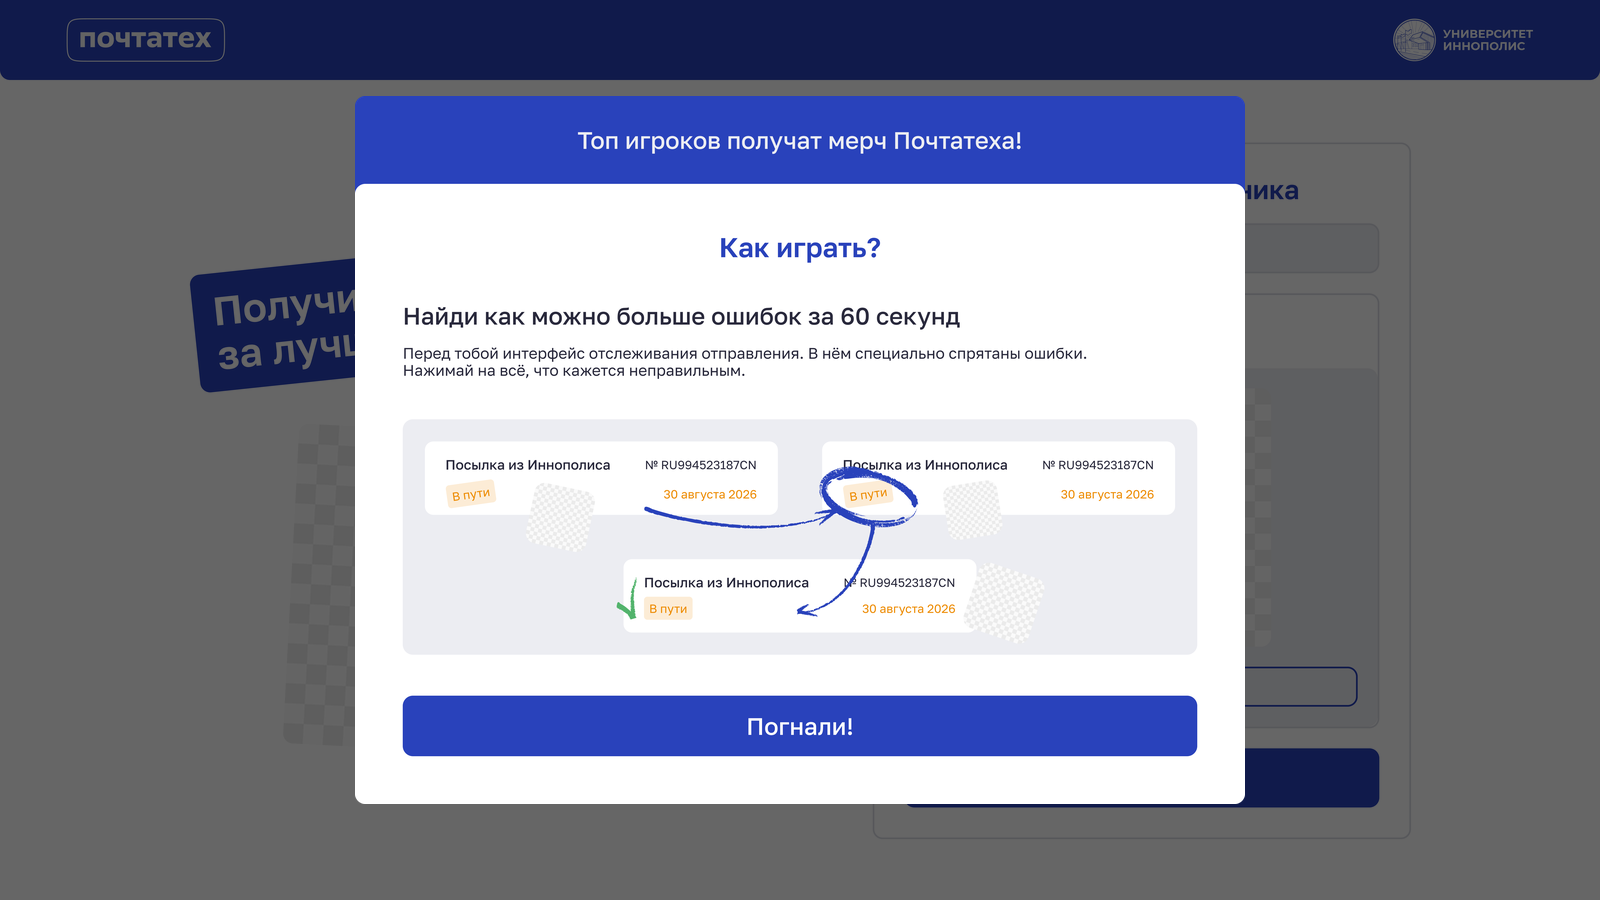
\includegraphics[width=0.48\textwidth]{../images/pochtatex/page2.png}%
  \hfill
  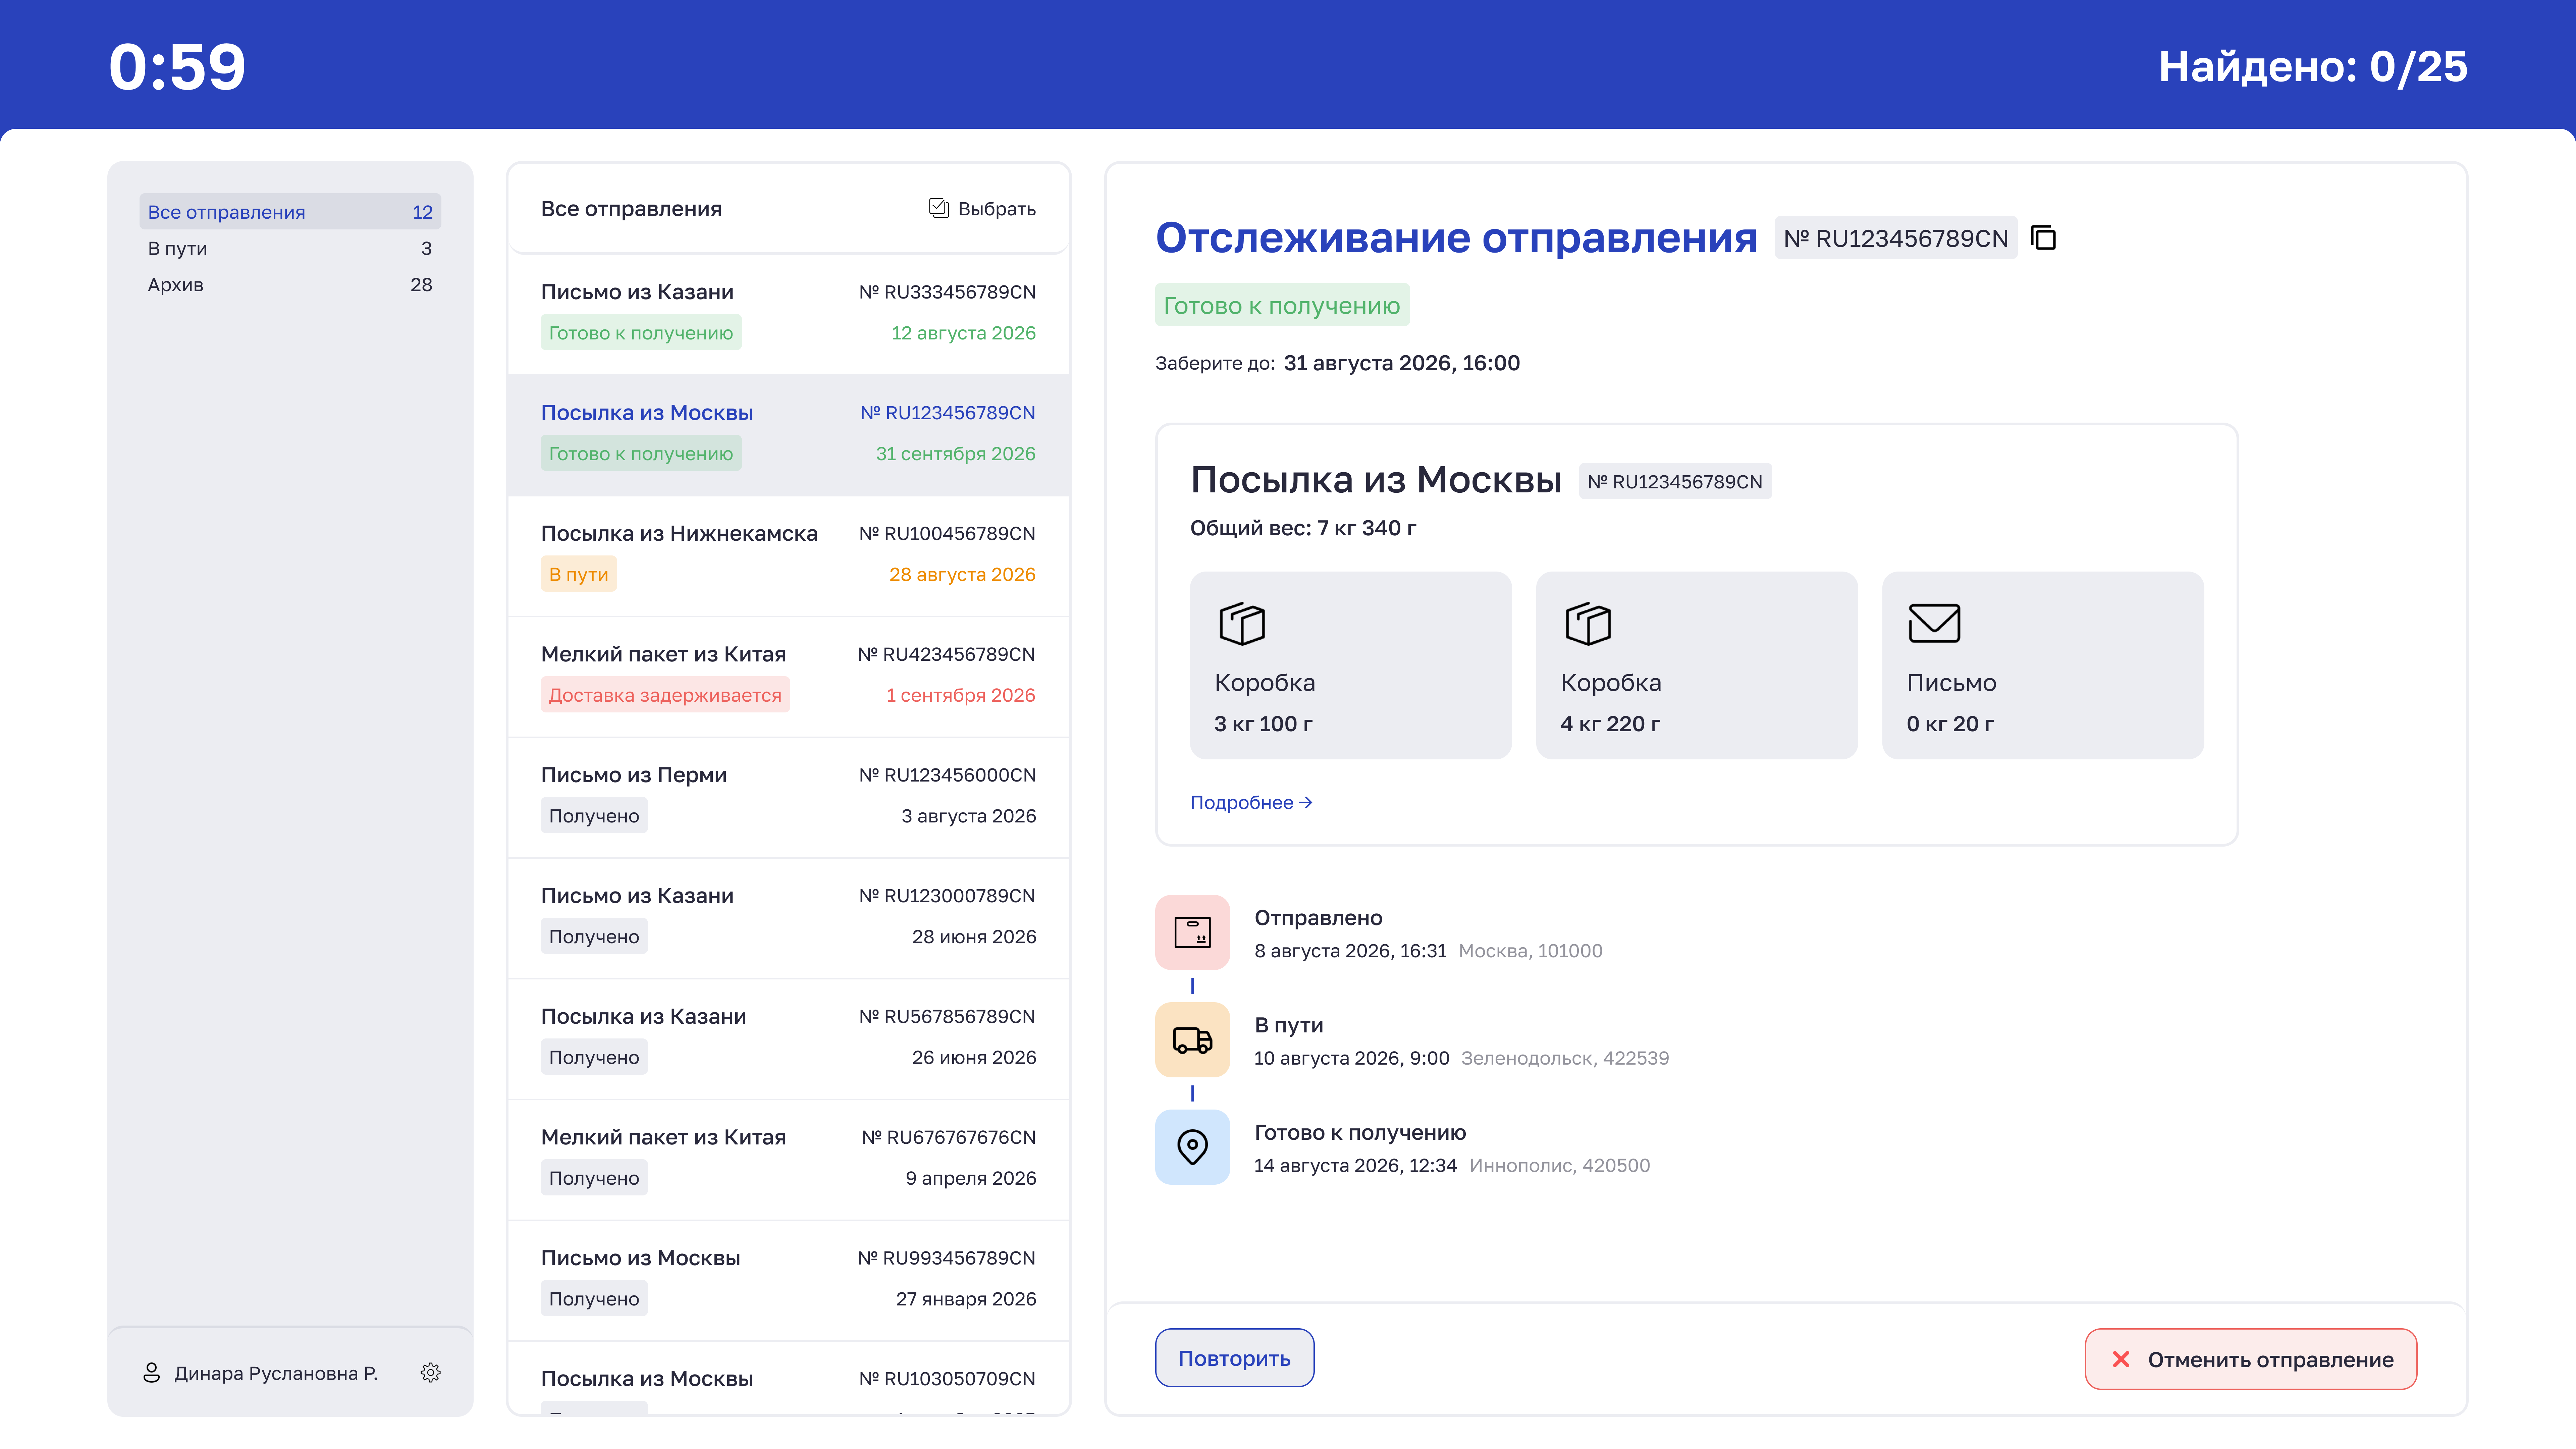
\includegraphics[width=0.48\textwidth]{../images/pochtatex/page3.png}
\end{center}
\begin{center}
  \textcolor{textgray}{\small Экраны игры · ПОЧТАТЕХ}
\end{center}

\project
{Croissan Studio}
{\href{https://croissanstudio.ru}{croissanstudio.ru} · in-house}
{
Визуальная экосистема AI-студии: логотип, мерч, иллюстрации и digital-носители для продукта «нейрохудожник». Задача --- связать бренд, мерч и интерфейсы в один узнаваемый язык.
}
{Figma, Adobe Illustrator, AI + ручная доработка}
{
\begin{itemize}
  \item Фирменные элементы, иллюстрации и носители в единой стилистике.
  \item Визуальный язык для продукта «нейрохудожник» и публичной витрины студии.
  \item Сочетание AI-генерации и ручной доработки.
\end{itemize}
}

\project
{Yoko Matcha}
{фриланс · интернет-магазин матчи}
{
Бренд должен ощущаться премиально, но тепло --- без холодного e-commerce шаблона. Выстроила палитру, типографику и сетку каталога; визуалы сгенерировала и доработала вручную под единый характер.
}
{Figma, AI-визуалы, UI e-commerce}
{
\begin{itemize}
  \item Дизайн главной, каталога и карточек товара в одной визуальной системе.
  \item Палитра, типографика и визуальный характер бренда.
  \item Макеты, готовые к передаче в сборку.
\end{itemize}
}

\project
{Барилова \& Царёв}
{Kingstep Dance Studio · \href{https://kingstep.ru}{kingstep.ru}}
{
Онлайн-школа танцев продаёт эмоцию и доверие к преподавателям, а не просто список курсов. Сделала сильный визуальный hero, структуру направлений и тёплую типографику; макет адаптировала под сборку в Tilda.
}
{Figma, Tilda, Adobe Illustrator}
{
\begin{itemize}
  \item Логика сайта: главная, каталог курсов, карточки занятий.
  \item Тёмная эстетика студии и согласование с брендом Kingstep.
  \item Макеты, промо-экраны и графика для сборки в Tilda.
\end{itemize}
}

\vspace{0.4em}
\begin{center}
  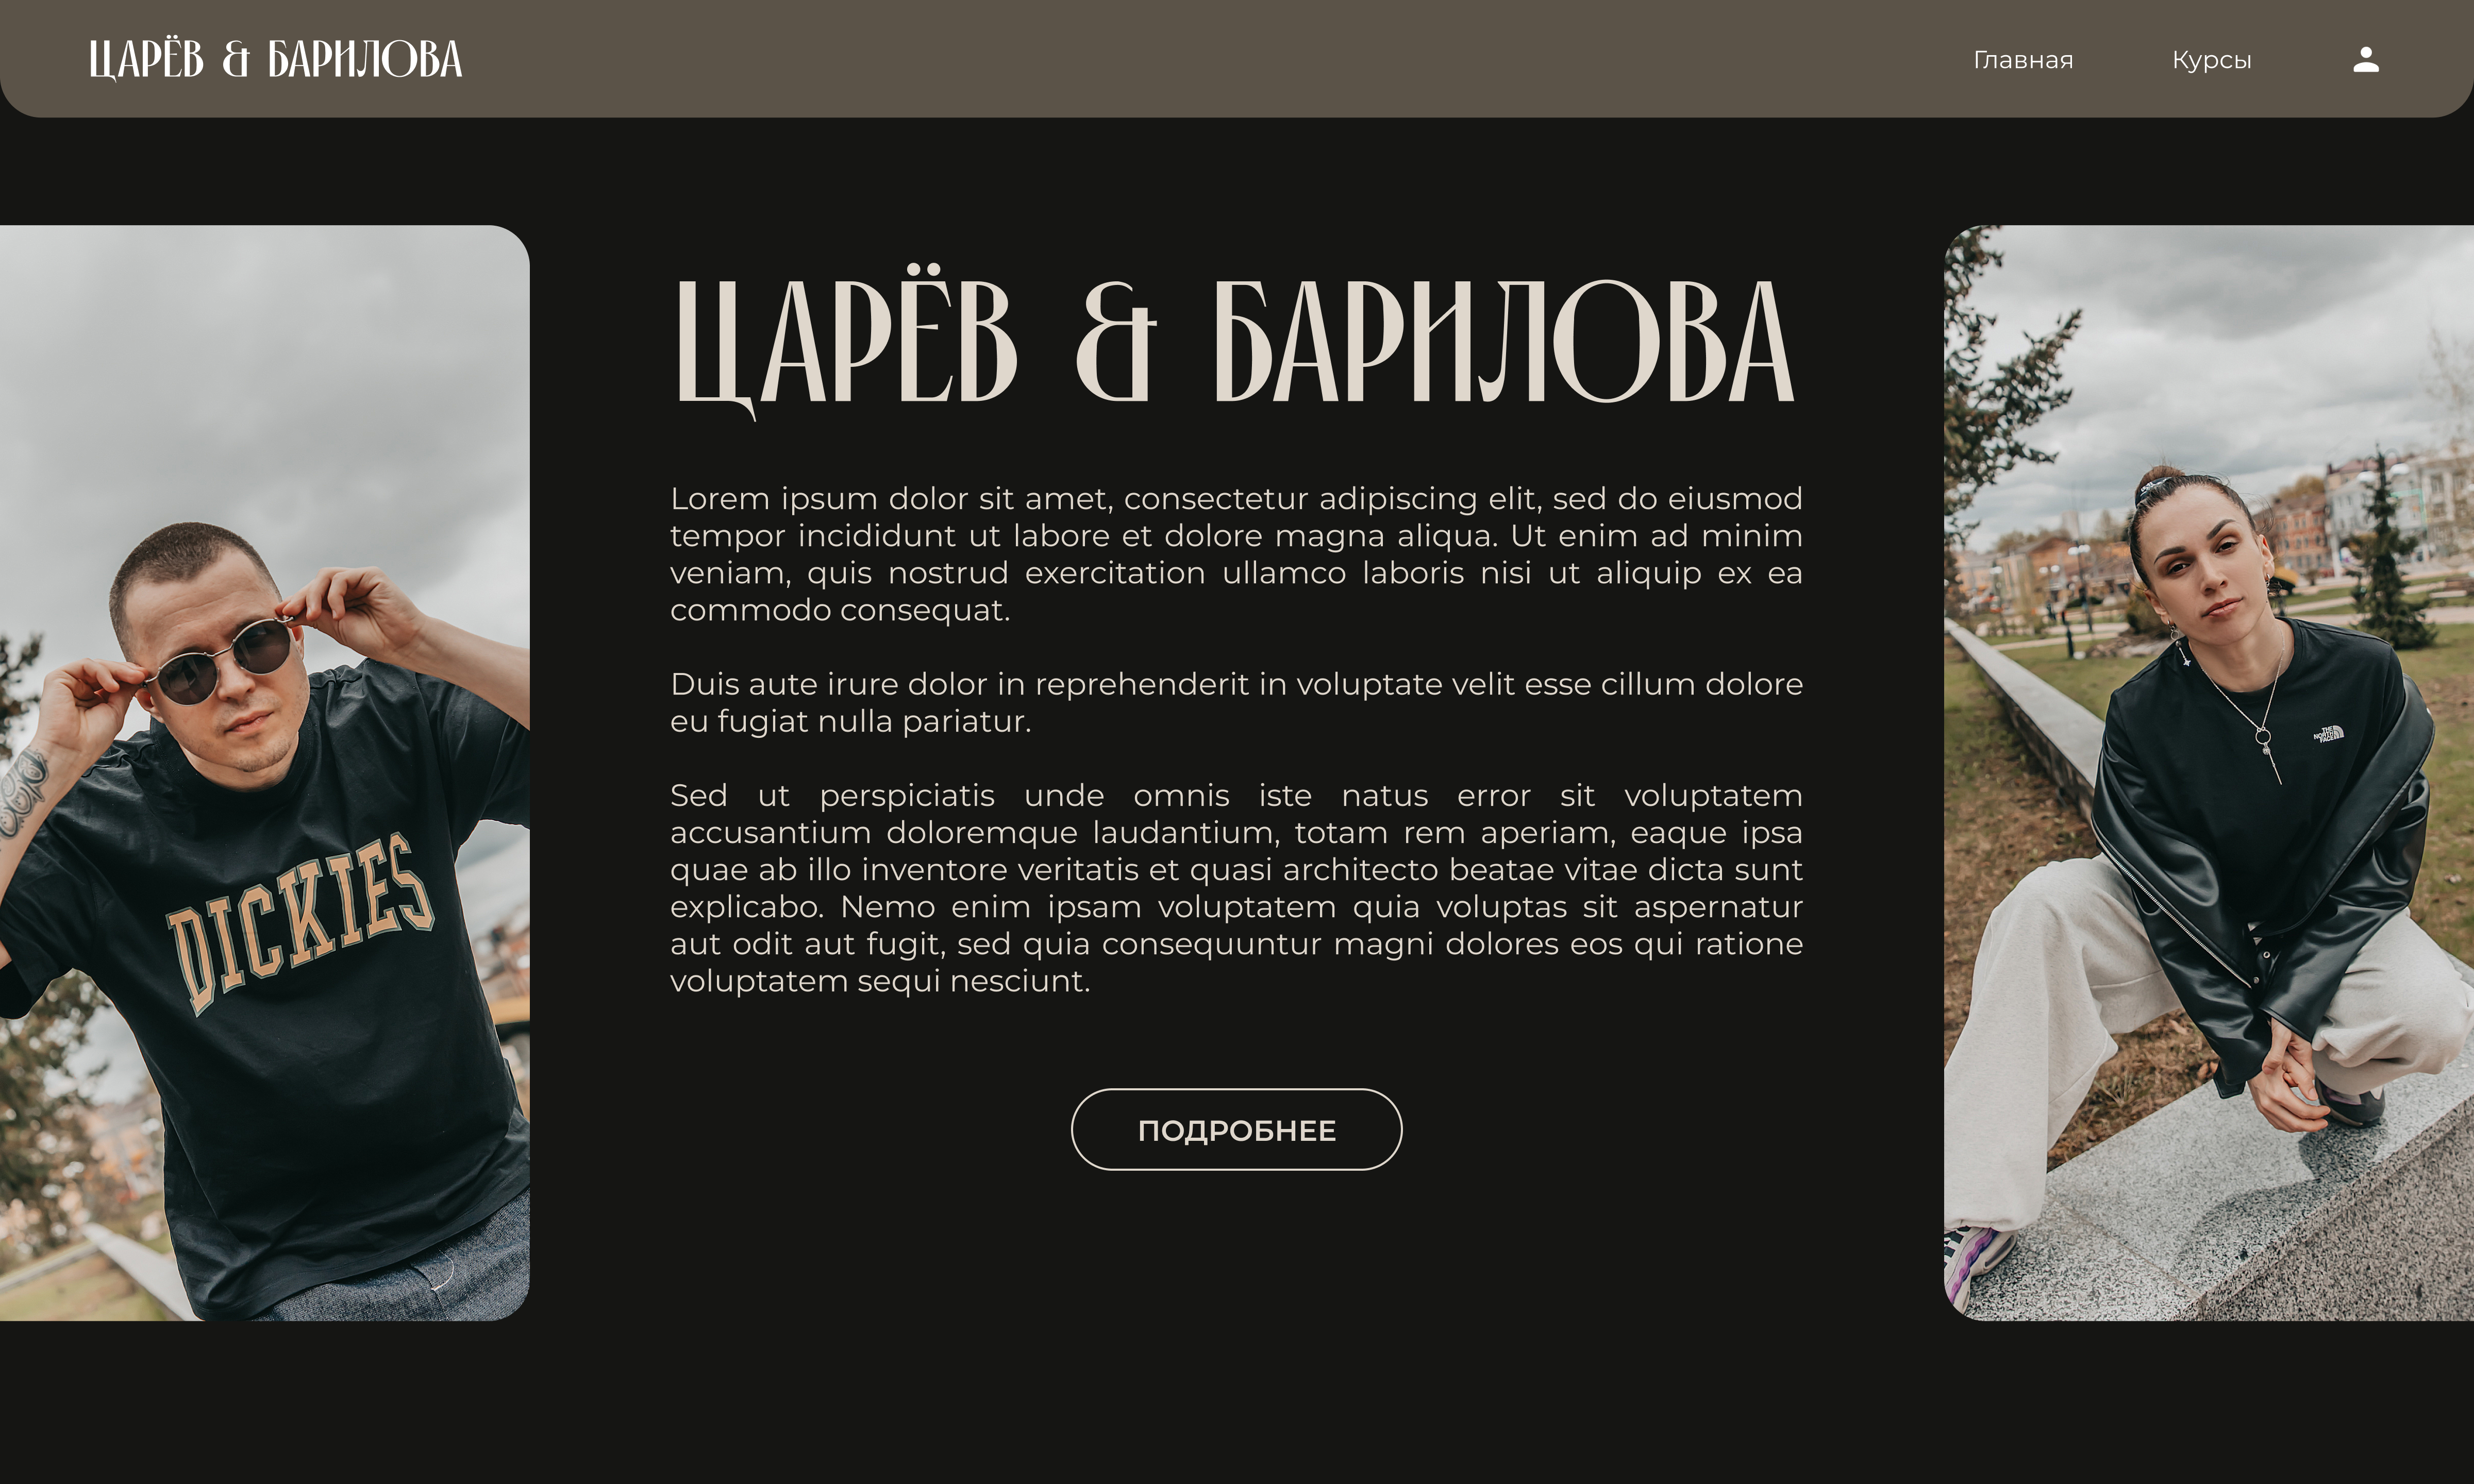
\includegraphics[width=0.48\textwidth]{../images/tsarevbarilova/page1.png}%
  \hfill
  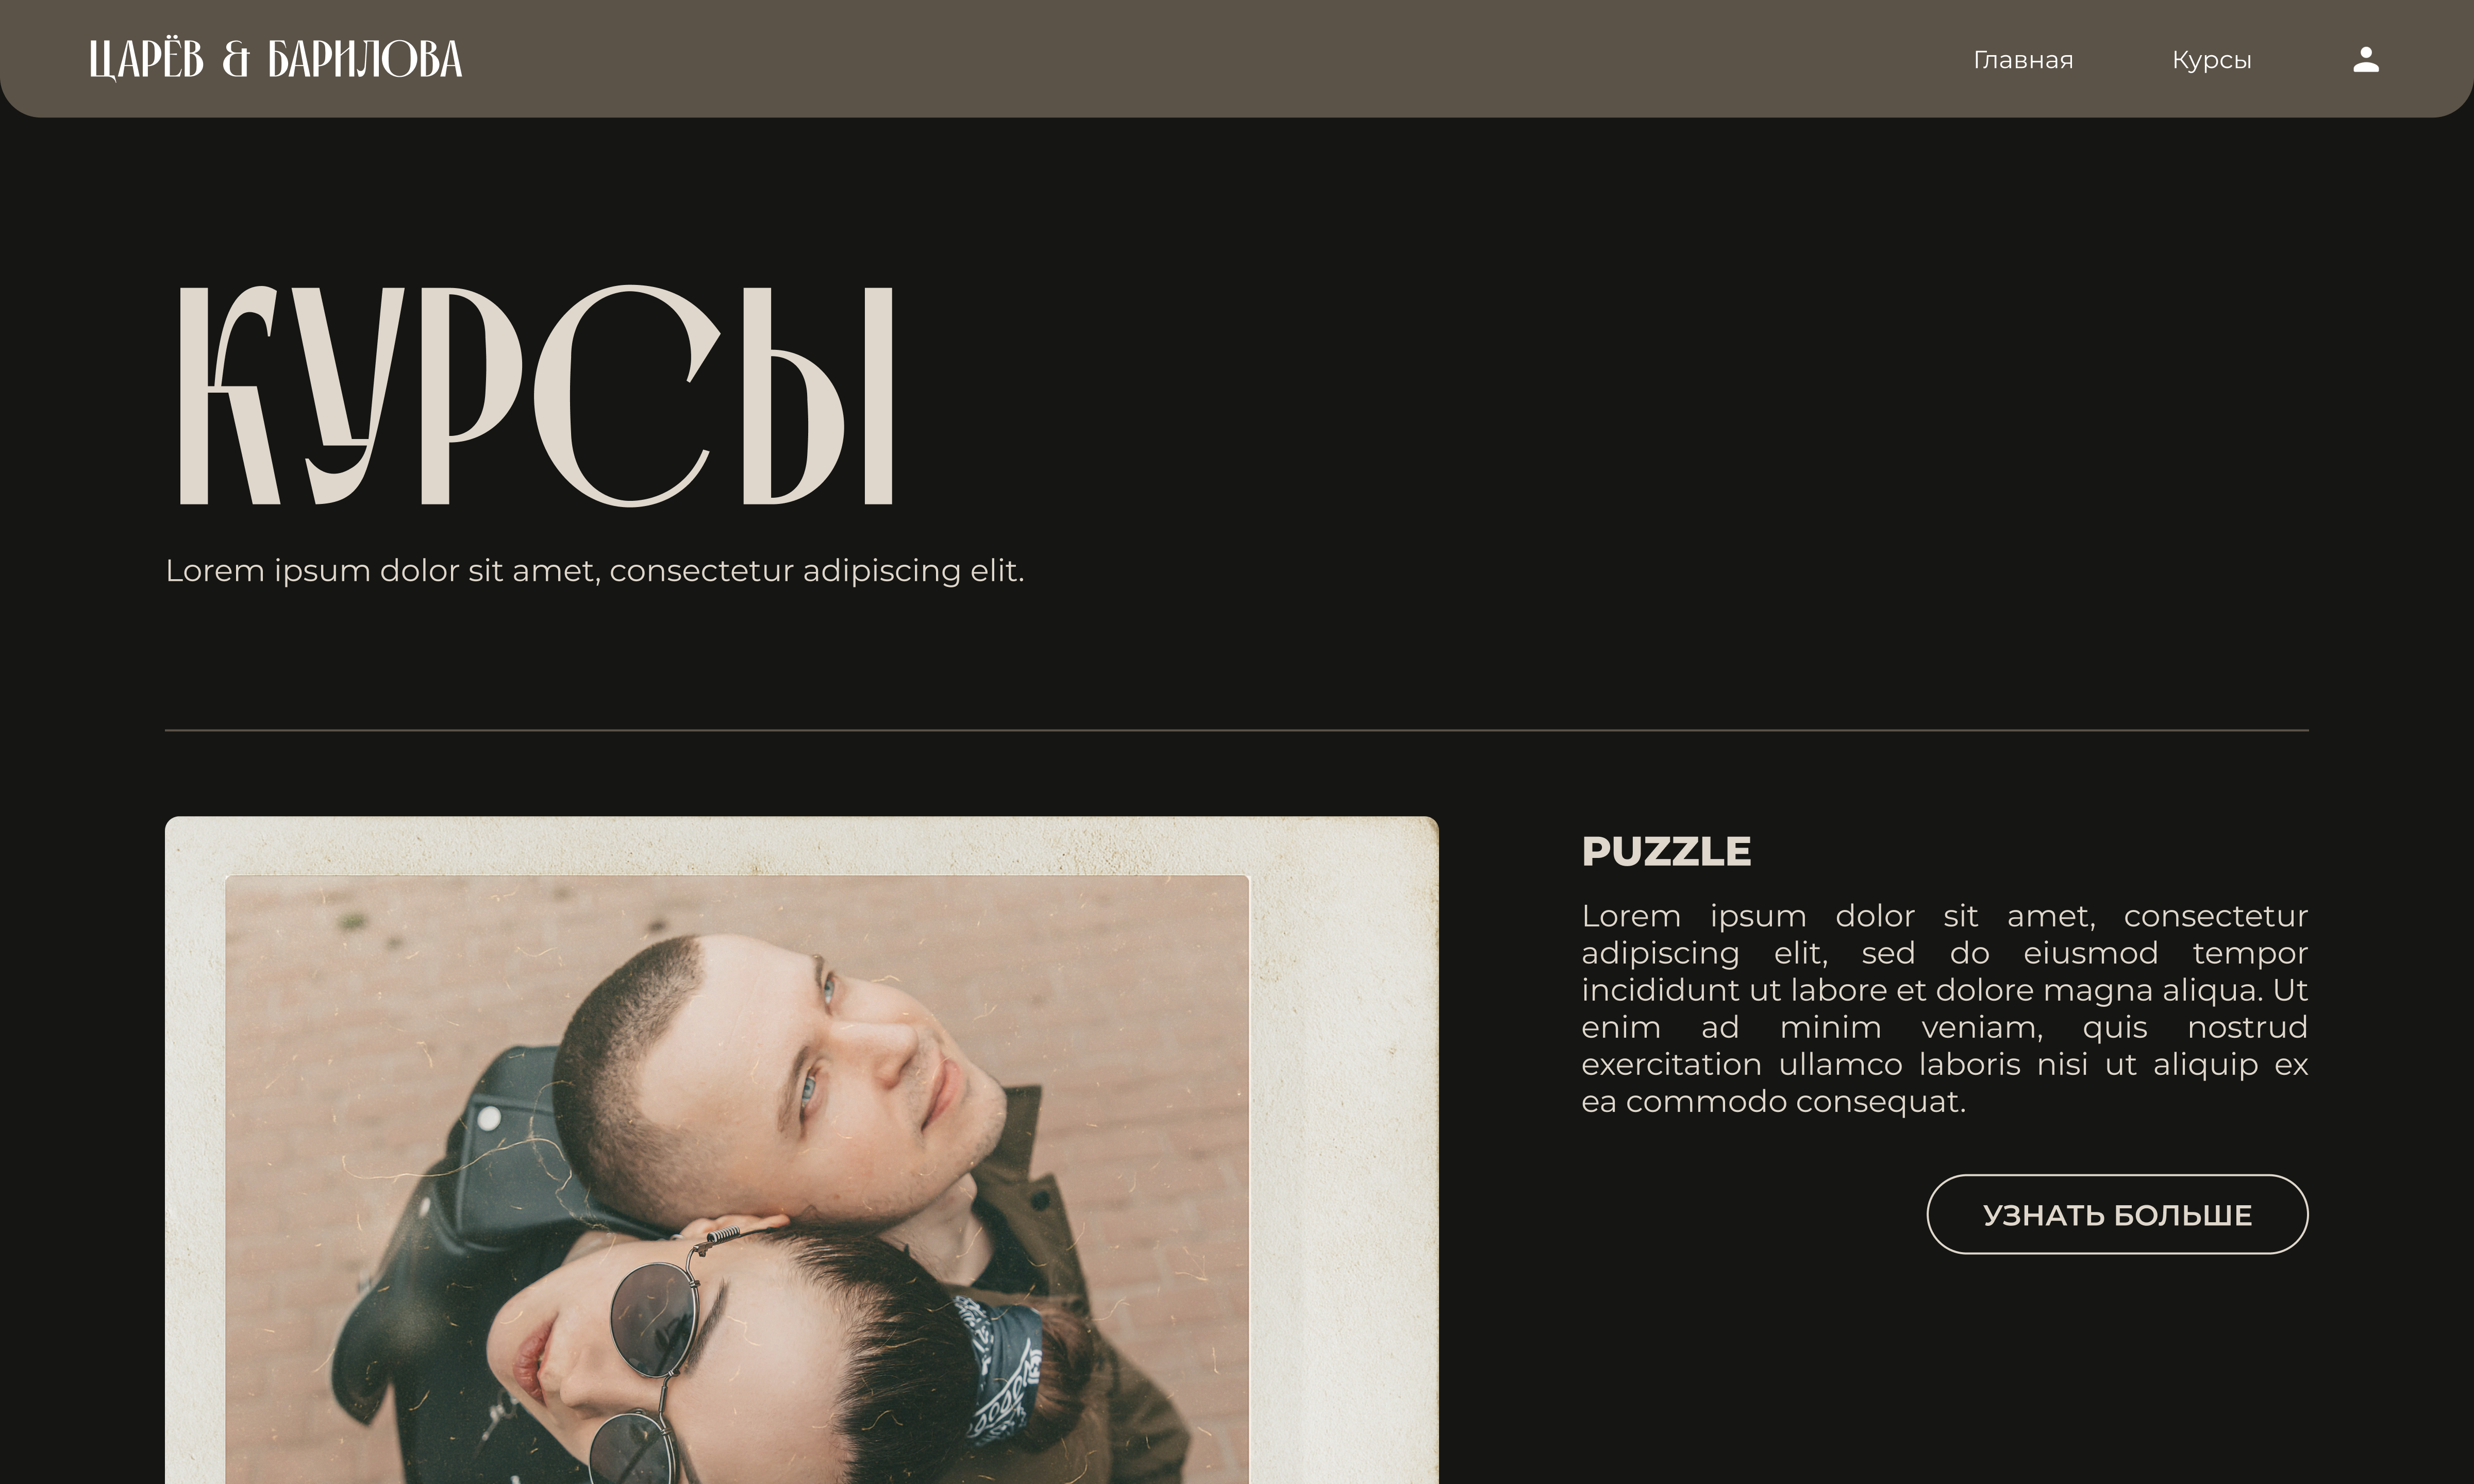
\includegraphics[width=0.48\textwidth]{../images/tsarevbarilova/page2.png}\\[0.5em]
  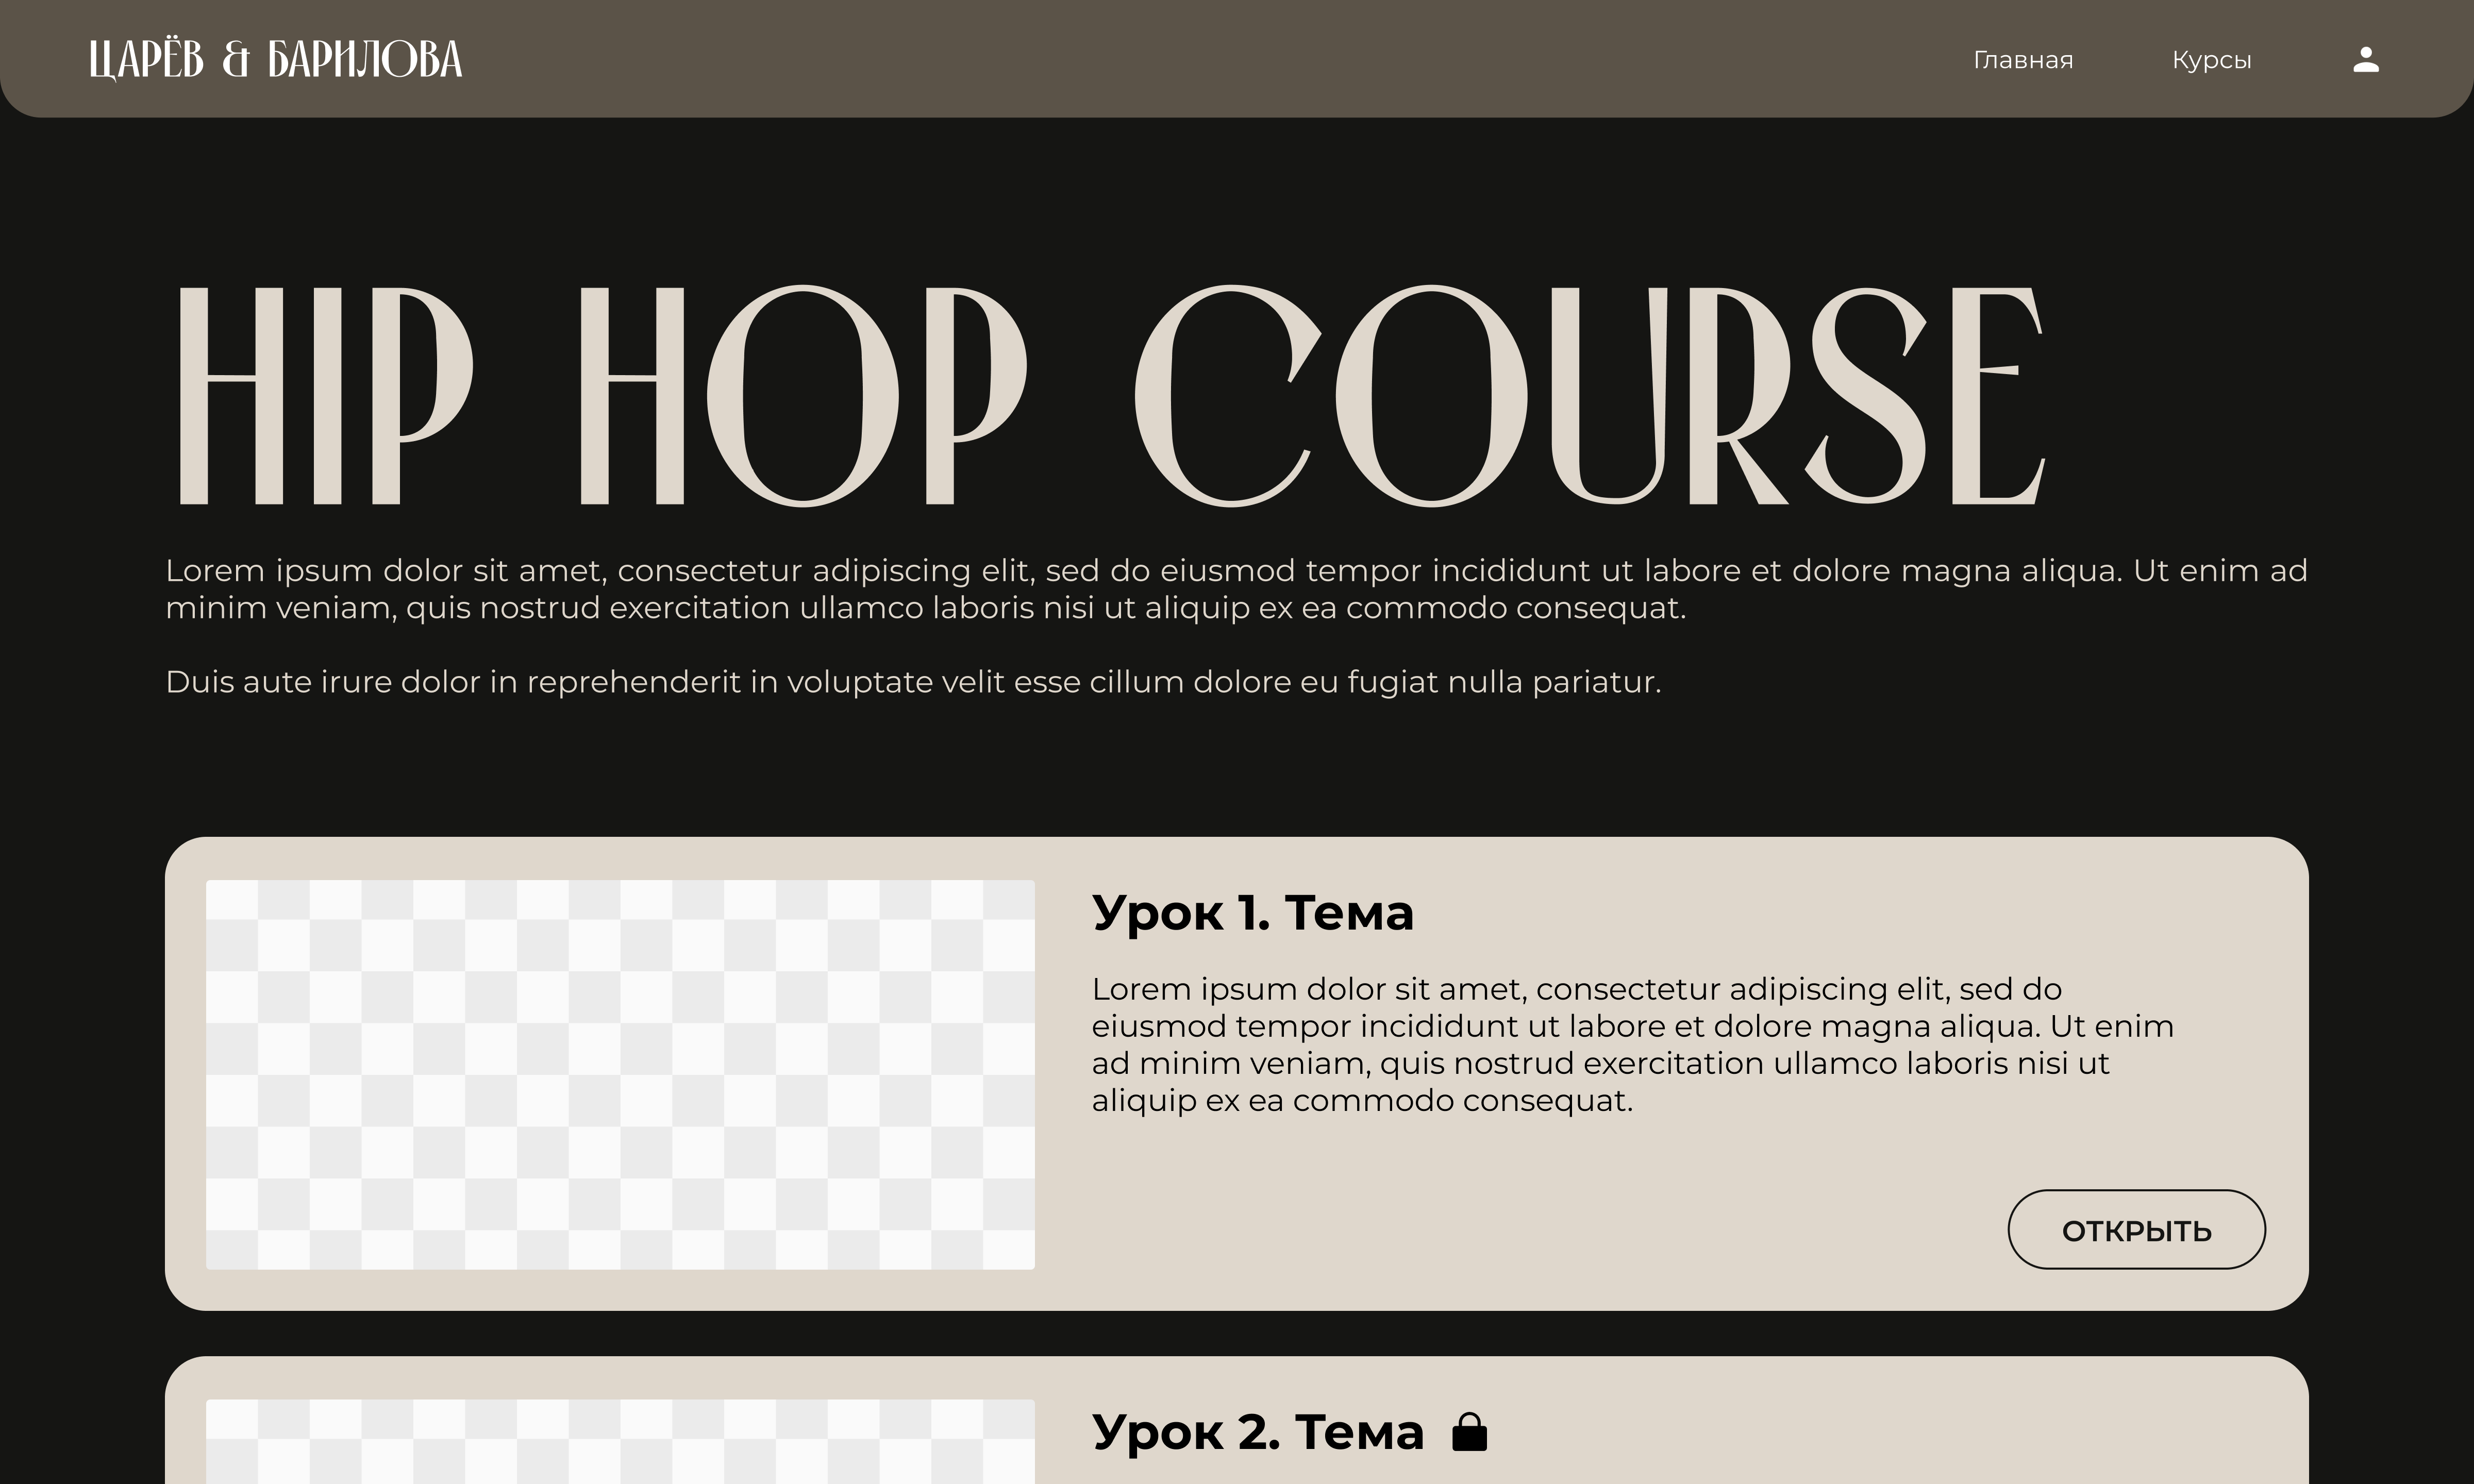
\includegraphics[width=0.48\textwidth]{../images/tsarevbarilova/page3.png}%
  \hfill
  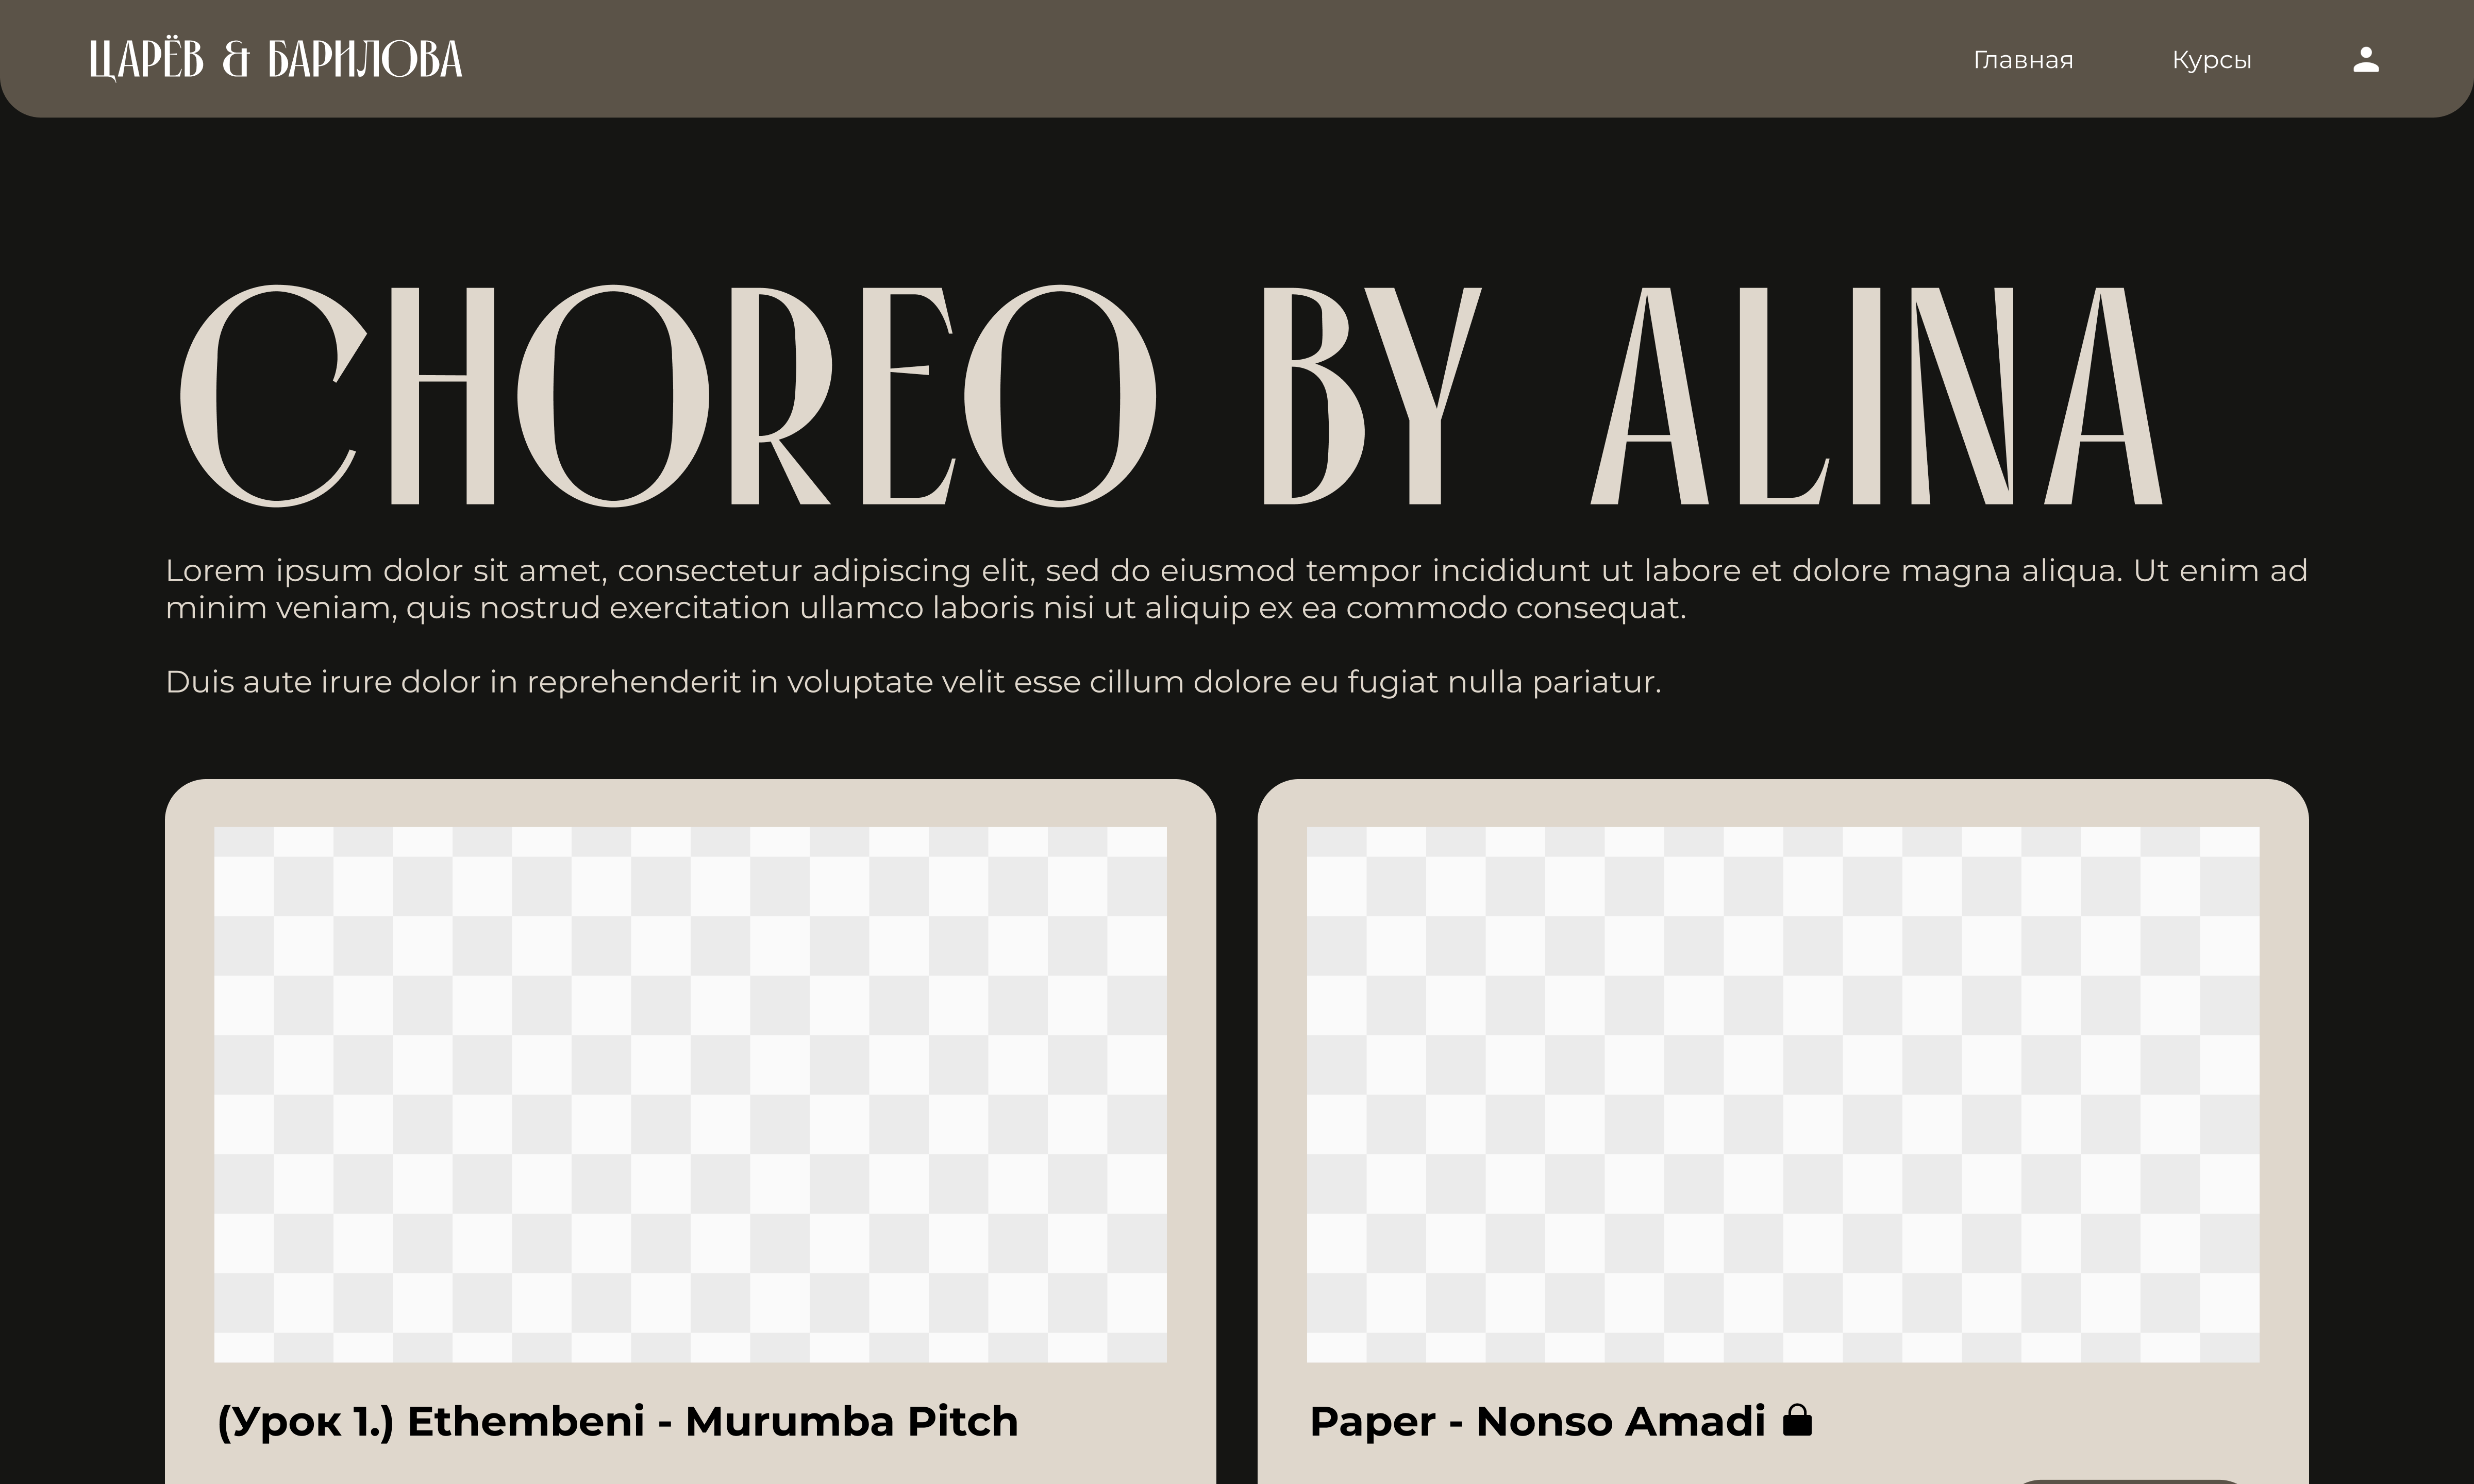
\includegraphics[width=0.48\textwidth]{../images/tsarevbarilova/page4.png}
\end{center}
\begin{center}
  \textcolor{textgray}{\small Ключевые экраны · Kingstep}
\end{center}

\project
{AI-смена · Иннополис}
{\href{https://aismena.ru}{aismena.ru}}
{
Лендинг летней AI-смены для школьников 7--11 классов: родитель должен понять программу и оставить заявку без звонка менеджеру. Собрала структуру, визуальную подачу и весь сайт на Tilda в сжатые сроки.
}
{Tilda, Zero Block, типографика, формы}
{
\begin{itemize}
  \item Hero, программа, расписание дня, команда, цена, FAQ и форма записи.
  \item Адаптивная вёрстка и иерархия контента под конверсию в заявку.
  \item Публикация на домене aismena.ru.
\end{itemize}
}

\project
{Постеры}
{ивенты Казани и Иннополиса}
{
Афиши для танцевальных и культурных мероприятий: должны цеплять с первого взгляда и оставаться читаемыми с расстояния и на экране телефона.
}
{Adobe Illustrator, Figma, AI}
{
\begin{itemize}
  \item Контраст, иерархия даты, места и названия, один сильный визуальный акцент.
  \item Афиши для танцевальных и культурных мероприятий в Казани и Иннополисе.
  \item Адаптация под печать и digital-распространение.
\end{itemize}
}

\section*{Как я работаю}

\begin{enumerate}
  \item Бриф: аудитория, цель продукта, ограничения по срокам и формату.
  \item Структура: user flow, приоритеты контента, ключевые экраны и CTA.
  \item Визуал: палитра, типографика, компоненты, mood и характер бренда.
  \item Прототип и макет: Figma или сборка в Tilda с учётом адаптива.
  \item Полировка: согласование, финальные правки, передача в разработку или публикацию.
\end{enumerate}

\section*{Дополнительно}

\begin{itemize}
  \item Технический бэкграунд: понимаю вёрстку и ограничения фронтенда при передаче макетов.
  \item Опыт в продуктовых командах: AzimovLab (AI-сервис генерации тестов), учебные продуктовые проекты в Иннополисе.
  \item ML / исследования: публикация по квантовым вычислениям (\textit{Вопросы кибербезопасности}, 2025).
\end{itemize}

\section*{Образование}

Университет Иннополис, бакалавриат «Прикладной искусственный интеллект», 2026.

\vfill

\begin{center}
\textcolor{textgray}{Последнее обновление: август 2026}
\end{center}

\end{document}
